In this chapter, we will review some of the critical elements of radiative transfer and radiative processes. These can be found more thoroughly treated in \textit{Rybicki \& Lightman} among others.

\section{Intensity and Other Definitions}

To begin, we need to clarify some definitions that are commonly used. We begin with \textbf{specific intensity}:
\vspace{0.5cm}
\begin{definition}[Specific Intensity]
The \textbf{specific intensity} $I_\nu(\mathbf{x}, \hat{\mathbf{n}}, t)$
is the energy transported by radiation per unit area, per unit time, per
unit frequency, per unit solid angle:
\[
    I_\nu \;\; \left[ \frac{\mathrm{erg}}
                          {\mathrm{s}\,\mathrm{cm}^2\,
                           \mathrm{Hz}\,\mathrm{sr}} \right].
\]
Formally,
\[
    dE = I_\nu \cos\theta \; dA \; dt \; d\nu \; d\Omega,
\]
where $\theta$ is the angle between $\hat{\mathbf{n}}$ (the propagation
direction) and the surface normal $dA$. \rmk{You can also write this with a dot product and $d{\bf A}$.}
\end{definition}
\vspace{0.5cm}
We are also quite interested in various \textbf{moments} of $I_\nu$ in order to generate other useful quantities:
\vspace{0.25cm}
\begin{definition}[Mean Intensity]
The \textbf{mean intensity} is the angle average of the specific
intensity:
\[
    J_\nu = \frac{1}{4\pi}\int I_\nu(\hat{\mathbf{n}})\, d\Omega,
    \qquad
    J_\nu \;\; \left[ \frac{\mathrm{erg}}
                          {\mathrm{s}\,\mathrm{cm}^2\,
                           \mathrm{Hz}\,\mathrm{sr}} \right].
\]
This quantity is isotropic by construction. It effectively counts the number of photons arriving at a point in space regardless of the direction.
\end{definition}
\vspace{0.25cm}
The \textbf{flux} is another common quantity, which ends up being the \textbf{first moment} of the specific intensity. Whereas intensity tells us how much energy we get from a particular direction, \textbf{flux tells us the total energy transfer from all directions}. Formally, we define the \textbf{flux vector} as
\vspace{0.25cm}
\begin{definition}[Flux]
    For a radiation field with specific intensity $I_\nu({\bf x},t, \hat{\bf n})$, the \textbf{flux vector} is 
\begin{equation}
        \boxed{
    {\bf F}_\nu = \int_{4\pi} I_\nu({\bf x},t,\hat{\bf n}) \hat{\bf n} \; d\Omega.
    }
\end{equation}
    If we then consider the quantity of energy passing through a surface $d{\bf A}$ in a unit time,
    \[
    dE_{\perp} = \int_{4\pi} d\Omega \; I_\nu (\hat{\bf n} \cdot d{\bf A}) = {\bf F}_\nu \cdot d{\bf A} = F_\nu \cos\theta dA.
    \]
\end{definition}

The first of these definitions encodes the direction of energy transfer, while the second describes how energy transfer occurs through a specific surface.
\par
We also distinguish between $\nu$-specific quantities and quantities integrated over $\nu$.
\vspace{0.25cm}
\begin{definition}[Bolometric vs. Monochromatic]
A \textbf{monochromatic} quantity is specified at a fixed frequency
$\nu$; for example, $I_\nu$ or $F_\nu$.  
A \textbf{bolometric} quantity is integrated over frequency:
\[
    I = \int_0^\infty I_\nu \, d\nu,
    \qquad
    F = \int_0^\infty F_\nu \, d\nu.
\]
Bolometric quantities therefore have units without the ``per Hz'' factor.
\end{definition}

\begin{definition}[Luminosity]
The \textbf{monochromatic luminosity} $L_\nu$ is the total power emitted
by a source per unit frequency:
\[
    L_\nu = \int_{\partial V} F_\nu \, dA,
    \qquad
    L_\nu \;\; \left[ \frac{\mathrm{erg}}
                          {\mathrm{s}\,\mathrm{Hz}} \right].
\]
The \textbf{bolometric luminosity} is
\[
    L = \int_0^\infty L_\nu \, d\nu
      = \int_{\partial V} F \, dA,
    \qquad
    L \;\; \left[ \frac{\mathrm{erg}}{\mathrm{s}} \right].
\]
\end{definition}
\par
The final integral over $I_\nu$ worth mentioning is the \textbf{energy density of radiation}:
Imagine that you hold a metal shield up to the sky in direction $\hat{\bf n}$. In some $dt$, a cone of photons will hit that shield. That cone of photons will have infinitesimal volume $c \; \cos \theta \;dAdt$. \rmk{the $\cos$ comes in because different cones see different cross sections.} Now, we know that the resulting energy that arrives at the shield is
\[
\delta E = I_\nu({\bf x},\hat{\bf n}) (\hat{\bf n} \cdot d{\bf A}) d\Omega d\nu dt.
\]
Within that region, there was
\[
u_\nu dV d\Omega d\nu
\]
energy, so setting these equal to one another,
\[
u_\nu(\hat{\bf n}) = \frac{1}{c} I_\nu({\bf x},\hat{\bf n}).
\]
If we integrate over all directions, we have
\begin{equation}
    \boxed{
    u_\nu = \frac{1}{c}\int_{4 \pi} I_\nu \;d\Omega = \frac{4\pi}{c} J_\nu,
    }
\end{equation}
where $J_\nu$ is the \textbf{average intensity}.


\section{Radiative Transfer}

Consider two disks a distance $dx$ apart with areas $dA_i$. Now, we are interested in the energy transfer of rays which pass through both screens. Consider first screen 1. A ray passing through screen one must be directed such that it points in the right direction to hit screen two, which has angular area $dA_2/dx^2$. Thus, the energy transfered along those rays is
\[
dE = I_{\nu,1} \;dA_1 dt d\Omega d\nu = I_{\nu,1} \frac{dA_1 dA_2}{dx^2} dt d\nu.
\]
Likewise, at screen 2, only those photons which passed through angular area $dA_1/dx^2$ could have passed through both, so
\[
dE = I_{\nu,2} \; dA_2 dt d\Omega d\nu \implies I_{\nu,1} = I_{\nu,2}.
\]
Thus, \textbf{intensity is conserved along rays}.
\par
There is however a caveat to this:

\begin{itemize}
    \item Light can be \textbf{scattered into a ray},
    \item Light can also be \textbf{emitted / absorbed} into a ray.
\end{itemize}

As such, there are some scenarios in which intensity along a ray is not constant.

\subsection{Emission}

Let's determine some of the nomenclature for emission mechanics. We define the \textbf{spontaneous emission coefficient} such that
\vspace{0.5cm}
\begin{definition}[Spontaneous Emission Coefficient]
\label{def:spont_emission_coef}
The \textbf{spontaneous emission coefficient} is the energy injected / emitted per unit time, per unit solid angle, and per unit volume. Thus
\[
dE = j(t,\hat{\bf n})\; dV d\Omega dt.
\]
\rmk{Note that this means the coefficient is a function of direction. This is the case for (say) Larmor radiation, which is not isotropic.}
\par
This can likewise be defined in terms of a \textbf{monochromatic emission coefficient} $j_\nu$, which is just the emission per unit frequency as well. Likewise, for \textbf{isotropic emission}, 
\[
dE = \int_{4\pi} d\Omega\; j_\nu dV dt = 4\pi j_\nu \; dV dt.
\]
Thus,
\[
P_\nu = \frac{j_\nu}{4\pi}
\]
is the \textbf{monochromatic power per unit volume.}
\end{definition}
\vspace{0.5cm}
We also often define another useful quantity which occurs in the context of \textbf{isotropic emission}:
\begin{definition}[Emissivity]
\
    The \textbf{emissivity} is the energy emitted per unit frequency, per unit mass, per unit time. It is thus \textbf{angle integrated}. Formally,
    \[
    dE = \epsilon_\nu \rho \; dV dt d\nu \frac{d\Omega}{4\pi}.
    \]
\end{definition}
\vspace{0.5cm}
By comparison to $j_\nu$, we see that 
\[
j_\nu = \frac{\epsilon_\nu \rho}{4\pi}.
\]
\paragraph{Added Intensity}
Having worked out all the definitions above, we want to know what the change in $dI_\nu$ is for a particular path $ds$. For an isotropic emitter,
\begin{equation}
\label{eq:emit_coeff}
    \boxed{
dI_\nu = j_\nu ds.
}
\end{equation}

\subsection{Absorption}
Unlike emission, where we are generally more interested in energy generation that we are in intensity specifically, for absorption, we simply \textit{define} absorption on the basis of decreasing intensity. Formally,
\vspace{0.5cm}
\begin{definition}[Absorption Coefficient]
The \textbf{absorption coefficient} is defined such that
\begin{equation}
\label{eq:absorb_coef}
\boxed{
    dI_\nu = -\alpha_\nu I_\nu ds.
    }
\end{equation}
Thus, it is the loss per unit intensity per unit length. 
\end{definition}
\vspace{0.5cm}
Now, it is generally good practice to connect $\alpha$ to a theoretical statement about the absorbers in question. Consider that a ray passes through an ambient space with a number density $n$ of absorbing particles, each of which has effective area $\sigma$. In a cylindrical region with area $dA$ and length $ds$, there are clearly $n \;dAds$ absorbers along the line of sight. Assuming that they are small enough that overlaps are unlikely, this would obscure some $n \sigma_\nu \; dAds$ of the available aperature. Now, \textbf{those particles absorb energy}:
\[
- dE = I_\nu \; dA_{\rm absorption}\;dt\;d\Omega\;d\nu = I_\nu (n \sigma_\nu dA dS) dt d\Omega d\nu.
\]
The intensity will also change because 
\[
-\Delta dE = - \Delta dI_\nu dA d\Omega dt d\nu = I_\nu (n\sigma_\nu dAds) dtd\omega d\nu.
\]
Cancelling terms, we find
\[
dI_\nu = -n\sigma_\nu I_\nu ds,
\]
so
\[
\boxed{
\alpha=n\sigma_\nu = \rho \kappa_\nu,
}
\]
where $\kappa$ is the \textbf{opacity.}
\begin{remark}
    One needs to be careful that this is valid since we require $\sigma_\nu^{1/2} \ll n^{-1/3}$ in order to not have issues with overlap and we also assume random distribution. This is \textbf{almost always the case}. Additionally, some things like stimulated emission are actually treated as part of the absorption since they are proportional to the intensity nonetheless.
\end{remark}
\subsection{The Equations of Radiative Transfer}

If we combine equations~\ref{eq:absorb_coef} and \ref{eq:emit_coeff}, we find the \textbf{classical radiative transfer equation}:
\begin{equation}
    \label{eq:radiative_transfer}
    \frac{dI_\nu}{ds} = -\alpha_\nu I_\nu + j_\nu.
\end{equation}
There are two special cases to consider before generating a fully formalized solution to the above equation:

\subsubsection*{Emission Only}
If the scenario without any absorption, we have $\alpha = 0$, so
\[
\boxed{
\frac{dI_\nu}{ds} = j_\nu \implies I_\nu = I_{\nu0} + \int_0^s j_\nu(\xi) \;d\xi.
}
\]
\rmk{So the increase in brightness is just the integral of the emission coefficient along the LOS.}
\subsubsection*{Absorption Only}
This one is a little trickier. We have
\[
\frac{dI_\nu}{ds} = -\alpha I_\nu.
\]
Formally, we have
\[
I_\nu(s) = I_\nu(0) \exp\left[-\int_0^s \alpha_\nu(\xi)\;d\xi\right].
\]
We may; however, make this solution somewhat simpler by introducing a \textit{dimensionless length scale}. We therefore introduce $d\tau = \alpha ds$ which then means that
\[
d\log I_\nu = -d\tau \implies I_\nu(\tau) = I_\nu(0) e^{-\tau},
\]
where we have implicitly set $\tau$ to be zero at our starting point. Formally,
\begin{equation}
    \label{eq:optical_depth}
    \boxed{
    \tau_\nu(s) = \int_0^s d\xi\; \alpha_\nu(\xi).
    }
\end{equation}
Now, if $I_\nu \propto \exp(-\tau)$, then we see that for $\tau \ll 1$, we have very little drop off and (for this particular sight line), the medium is \textbf{transparent}. Likewise, if $\tau \gg 1$, then it is \textbf{optically-thick} or \textbf{opaque.}

\subsubsection*{The Formal Solution}
Let's return to
\[
\frac{dI_\nu}{ds} = -\alpha_\nu I_\nu + j_\nu.
\]
in the $\tau$ coordinate system,
\[
\frac{1}{\alpha_\nu} \frac{dI_\nu}{ds} = \frac{dI_\nu}{d\tau} = -I_\nu + S_\nu,
\]
where $S_\nu = j_\nu/\alpha_\nu$ is the \textbf{source term}. Now, this may be solved by an integrating factor, so
\[
\left(\frac{dI_\nu}{d\tau} + I_\nu\right)e^\tau = \frac{d}{d\tau} \left(e^\tau I_\nu\right) = e^\tau S_\nu.
\]
As such,
\[
e^\tau I_\nu = I_\nu(0) +\int_0^\tau d\xi \;S_\nu(\xi) e^\xi, 
\]
so
\[
\boxed{
I_\nu(\tau) = I_{\nu,0}e^{-\tau} + \int_0^\tau d\xi \; S_\nu(\xi) e^{\xi-\tau}.
}
\]
\subsection{The Mean Free Path}

In a medium with \textbf{no sources}, the equation above suggests that
\[
I_\nu(\tau) = I_{\nu,0} e^{-\tau}.
\]
Since the intensity encodes the number of photons effectively passing through a region, we see that
\[
P_{\rm collision} = \frac{I_\nu}{I_{\nu,0}} = e^{-\tau}.
\]
We can then ask what the average distance before collision will be. Clearly,
\[
\left<\tau\right> = \int_0^\infty \tau e^{-\tau} d\tau = 1 \implies \left<\ell\right> = (1/\alpha_\nu) = 1/(n\sigma_\nu).
\]
This quantity is then the \textbf{mean free path} of the photons between collisions.

\subsection{Radiation Force}
We have already discussed the advent of radiation pressure in a photon gas. We also need to acknowledge that when photons are absorbed in a particular ray, they will experience a force. Recall that the energy flux vector is
\[
{\bf F}_\nu = \int I_\nu \hat{\bf n} \;d\Omega.
\]
Thus,
\[
\frac{d{\bf F}_\nu}{d\tau} = \int \frac{\partial I_\nu}{\partial \tau} \hat{\bf n}\; d\Omega = - \int I_\nu \hat{\bf n} \;d\Omega = -{\bf F}_\nu. 
\]
\rmk{This makes NO SENSE except when you realize $d\tau = \alpha ds$, so if there is no absorption, your parameter doesn't even progress.} We can also write this as 
\[
\frac{d{\bf F}_\nu}{ds} = -\alpha {\bf F_\nu} \implies \frac{d{\bf p}_\nu}{ds} = -\frac{\alpha}{c} {\bf F}_\nu.
\]
Now, this is the \textbf{momentum}, but it is per unit area and per unit path length. But that's just \textbf{momentum density}. We can therefore identify the \textbf{force per unit mass} to be
\[
{\bf f} = \frac{1}{c} \int \kappa_\nu {\bf F}_\nu \;d\nu.
\]

\section{Thermal Radiation}

In this section we study the properties of emission from \textbf{thermally equilibrated material}. 

\subsection{Kirchhoff's Law}

Our first step is to understand how the notion of \textbf{local thermal equilibrium} (LTE) constrains the interaction of matter with radiation. This will lead us to two results collectively known as \textbf{Kirchhoff's Law}. 

\begin{center}
    Imagine a chamber filled with a \textbf{photon gas} in thermal equilibrium at temperature $T$. Now place this chamber in contact with another chamber, also at temperature $T$, but whose walls are made of material that can absorb and emit radiation.
\end{center}

If, at some frequency $\nu$, the two chambers had different intensities $I_{\nu,1} \neq I_{\nu,2}$, there would be a net transfer of photons at that frequency. This would imply a net flow of energy between two systems at the same temperature, in violation of the second law of thermodynamics. Therefore, microscopic absorption and emission must balance in such a way that the radiation field is not disturbed. 

\begin{theorem}[Kirchhoff's Law \#1]
For material in local thermal equilibrium at temperature $T$, the ratio of the emission coefficient to the absorption coefficient is universal and equals the Planck function:
\[
\frac{j_\nu}{\alpha_\nu} = B_\nu(T),
\]
Equivalently, the source function
\[
S_\nu \;\equiv\; \frac{j_\nu}{\alpha_\nu}
\]
is equal to the blackbody intensity at temperature $T$.
\end{theorem}

\begin{remark}
There is an important distinction between \emph{blackbody radiation} and \emph{thermal emission}. 
\begin{itemize}
    \item In a closed cavity where both matter and radiation are in \textbf{global equilibrium}, the radiation field itself must be Planckian:
    \[
    I_\nu = B_\nu(T), \qquad S_\nu = B_\nu(T).
    \]
    This is the defining property of blackbody radiation. 

    \item In contrast, in many astrophysical systems (e.g. stellar atmospheres), the material may be in LTE while the radiation field is not. In this case we still have
    \[
    S_\nu = B_\nu(T),
    \]
    but the actual intensity $I_\nu$ is determined by solving the radiative transfer equation with this source function and the boundary conditions. In general,
    \[
    I_\nu \neq B_\nu(T).
    \]
\end{itemize}
Thus, Kirchhoff's law fixes the form of the \emph{source function}, but only in global equilibrium does the radiation field itself become blackbody.
\end{remark}
\subsection{The Planck Distribution}
We may now endeavor to understand this $B_\nu(T)$ that we have such need of. This will lead us to the \textbf{plank distribution}, which is derived from statistical mechanics. The \textbf{photon gas} has the distinctive property that it is composed of a set of effectively non-interacting bosons. As such, each quantum state is \textbf{independently equilibrated}. A state may therefore have energy $\mathcal{E}$ and $N$ particles within it and can exchange both of these quantities with the rest of the environment. This is therefore a \textbf{grand-canonical ensemble}. The partition function is
\[
\mathcal{Z} = \sum_N \exp(N(\mu - \mathcal{E})\beta).
\]
Now, because these are bosons, there is no upper limit on $N$ as we have for fermions, so we can simply sum this as a geometric series.
\[
\mathcal{Z} = \frac{1}{1-\exp\left[(\mu - \mathcal{E})\beta\right]}.
\]
For photons, the chemical potential is $\mu = 0$, and so the mean occupation of a single mode is
\[
\left<N\right> = \frac{1}{1-\exp(h\nu \beta)}
\]
Now, the question becomes how many modes are there in a particular volume? We characterize a mode by ${\bf n} = (n_1,n_2,n_3)$ and recall that
\[
\mathcal{E} = \frac{hc}{2L} |{\bf n}| \implies d\mathcal{E} = \frac{hc}{2L} dn.
\]
If the density of states $g(\nu)$ is known, then 
\[
g(\nu) d \nu = \pi n^2 dn = \frac{8\pi L^3}{h^3c^3} \mathcal{E}^2 d\mathcal{E} = \frac{8\pi L^3}{c^3} \nu^2 d\nu.
\]
Combining this with the occupation probability yields
\begin{equation}
    \label{eq:bb_radiance}
    \boxed{
    B_\nu(T) = I_\nu(T) = \frac{c}{4\pi} u_\nu(T) = \frac{2 h \nu^3}{c^2} \frac{1}{e^{h\nu/k_bT} -1}.
}
\end{equation}
\subsubsection{Properties of the Plank Distribution}

Here we summarize some critical results from the Plank Distribution:
\vspace{0.25cm}
\begin{definition}[Rayleigh-Jeans Law]
For $h\nu \ll k_bT$, 

\begin{equation}
\label{eq:Rayleigh-Jeans}
\boxed{
I_\nu(T) =  \frac{2\nu^2}{c^2} kT.
}
\end{equation}
\end{definition}
\begin{proof}
    For $h\nu \ll k_bT$, $\exp(h\nu/k_bT) \approx 1+ (h\nu/k_bT)$, so we find the above result.
\end{proof}
\begin{remark}
    This is very useful for a couple of reasons. First off, it allows you to recover Planck if you remember how RJ comes about and how the exponential term should look. Secondly, for \textbf{low frequency radiation}, this approximation is almost always legitimate and is linear in $\nu$.
\end{remark}
\vspace{0.25cm}
In the \textbf{high frequency limit}, we have an equivalent result called \textbf{Wein's Law}:
\vspace{0.25cm}
\begin{definition}[Wein's Law]
    For $h\nu \gg k_bT$, we have
    \begin{equation}
        \label{eq:Wein-Law}
            I_\nu(T) = \frac{2h \nu^3}{c^2} \exp\left(\frac{-h\nu}{kT}\right).
    \end{equation}
\end{definition}
\vspace{0.25cm}
We also have the following two useful propositions:
\vspace{0.1cm}
\begin{proposition}[Monotonicity]
Let $T_1$ and $T_2$ be temperatures. $T_1 > T_2$ implies that $I_\nu(T_1) > I_\nu(T_2)$ for all $\nu$.
\end{proposition}
\begin{proof}
    This is done simply by taking the derivative with respect to $T$ and showing that it is always positive.
\end{proof}

\begin{proposition}[Wein's Offset Law]
The \textbf{peak frequency} $\nu_{\rm max}$ is such that
\[
h\nu_{\rm max} = 2.82\; kT.
\]
\end{proposition}

\subsection{Thermodynamics of BB Radiation}
As we have previously discussed, emission and absorption from the barriers of the container can serve to thermalize light into a blackbody spectrum. If we then compress or expand the cavity, we have thermodynamic work from which we can gain great insight. First off
\[
dU = TdS - pdV \implies dS = \frac{1}{T}dU + \frac{p}{T} dV.
\]
We know, however, that $p = u/3$ from arguments made about the photon gas, and we know that $U=u(T) V$, so
\[
dS = \frac{1}{T}\left[u dV + Vdu\right] + \frac{1}{3}\frac{u}{T} dV =\frac{4}{3} \frac{u}{T} dV + \frac{V}{T}du.
\]
now, $S$ is a function of $T$ and $V$, so
\[
ds = \left(\frac{\partial u}{\partial T}\right)_V dT + \left(\frac{\partial u}{\partial V}\right)_T dV.
\]
As such,
\[
\frac{\partial^2 S}{\partial T \partial V} = -\frac{4}{3}\frac{u}{T^2} + \frac{4}{3} \frac{1}{T} \frac{\partial u}{\partial T} =  \frac{1}{T}\frac{du}{dT}.
\]
The result is that
\[
\frac{du}{u} = 4 \frac{dT}{T} \implies \log u = 4 \log T +\log a.
\]
This is the \textbf{steffan-Boltzmann Law}:
\[
u(T) = aT^4,
\]
where $a$ is the \textbf{radiation constant}. We may likewise calculate the \textbf{flux} as
\[
F = \sigma T^4.
\]

\subsection{Characteristic Temperatures}

Several characteristic temperatures are defined in relation to thermal emission.  
They allow us to compare real sources with the idealized behavior of a blackbody.

\vspace{0.5cm}
\begin{definition}[Brightness Temperature]
The \textbf{brightness temperature} $T_b(\nu)$ is the temperature a blackbody would need to have in order to produce the same specific intensity at a given frequency $\nu$:
\[
I_\nu = B_\nu\!\left(T_b(\nu)\right).
\]
Since the definition is frequency–dependent, $T_b$ is in general a function of $\nu$.
\end{definition}

\vspace{0.3cm}
\begin{definition}[Color Temperature]
The \textbf{color temperature} $T_c$ is the temperature of a blackbody whose spectrum peaks at the same frequency (or wavelength) as the observed source, i.e.
\[
\nu_{\rm max}^{\rm source} = \nu_{\rm max}^{\rm BB}(T_c).
\]
\end{definition}

\vspace{0.3cm}
\begin{definition}[Effective Temperature]
The \textbf{effective temperature} $T_{\rm eff}$ is the temperature of a blackbody that would produce the same total flux as the source.  
For a source with bolometric flux $F$,
\[
F = \int I_\nu \cos\theta \, d\Omega \, d\nu = \sigma T_{\rm eff}^4.
\]
\end{definition}
\par
There are a few remarks worth making about these temperature measures:
\vspace{0.2cm}
\begin{itemize}
    \item \textbf{Brightness temperature $T_b(\nu)$.}  
    In the radio regime, the Rayleigh–Jeans approximation to the Planck function applies:
    \[
    B_\nu(T) \approx \frac{2\nu^2 k_B T}{c^2}.
    \]
    Using the definition $I_\nu = B_\nu(T_b)$, this gives
    \[
    T_b(\nu) \;\approx\; \frac{c^2}{2k_B \nu^2} I_\nu.
    \]
    Thus, $T_b$ can be obtained directly from a measured intensity $I_\nu$ by a simple algebraic inversion.  
    This is one of the main reasons $T_b$ is widely used in radio astronomy.
    
    \item \textbf{Color temperature $T_c$.}  
    $T_c$ depends only on the \emph{shape} of the spectrum, since it is defined by the location of the emission maximum.  
    For a blackbody, Wien’s displacement law gives
    \[
    \nu_{\rm max} \propto T_c, \qquad \lambda_{\rm max} T_c = b,
    \]
    with $b \approx 2.9 \times 10^{-3}\,\mathrm{m \, K}$.  
    Because the peak is a function of spectral shape alone, $T_c$ is insensitive to the overall flux normalization.

    \item \textbf{Effective temperature $T_{\rm eff}$.}  
    $T_{\rm eff}$ encodes the total radiated power, independent of spectral details.  
    For a source of luminosity $L$ and radius $R$,
    \[
    F = \frac{L}{4\pi R^2} = \sigma T_{\rm eff}^4,
    \]
    where $F$ is the bolometric flux at the surface.  
    This makes $T_{\rm eff}$ the standard measure for stellar classification and energy output.
\end{itemize}

\section{Electron Scattering}

In this section, we briefly touch on the details of \textbf{Thompson scattering} and its relativistic counterpart \textbf{Compton scattering}. 

\subsection{Thompson Scattering}

\begin{definition}[Thomson Scattering]
    \label{def:thomson_scattering}
    \textbf{Thomson scattering} is the non--relativistic limit of the
    scattering of an incident electromagnetic wave off of a free
    electron.
\end{definition}

\noindent
Consider an incident plane electromagnetic wave,
\[
    {\bf E}({\bf x},t) = E_0 \exp\!\left[i({\bf k}\cdot{\bf x} - \omega t)\right]\boldsymbol{\epsilon},
\]
where $\boldsymbol{\epsilon}$ is the polarization vector of the incoming
wave. In the non--relativistic limit ($\beta \ll 1$), the Lorentz force
reduces to
\[
    {\bf F}_{\rm Lorentz} = q\left({\bf E} + \frac{\mathbf{v}}{c}\times {\bf B}\right)
    \approx q{\bf E},
\]
so that the electron’s equation of motion is
\[
    m\ddot{\bf r} = q{\bf E} \qquad \implies \qquad
    \ddot{\bf d} = \frac{q^2}{m}{\bf E},
\]
where ${\bf d} = q{\bf r}$ is the electric dipole moment of the electron.
Integrating twice gives
\[
    {\bf d}(t) = -\frac{q^2}{m\omega^2}{\bf E}(t),
\]
so the electron behaves as an oscillating dipole of frequency $\omega$
and amplitude
\[
    {\bf d}_0 = \frac{q^2E_0}{m\omega^2}\,\boldsymbol{\epsilon}.
\]
\begin{remark}
    The dipole oscillation is \textbf{coherent} with the polarization of
    the incident wave: the electron is driven along
    $\boldsymbol{\epsilon}$.
\end{remark}

\noindent
For a sinusoidal oscillation ${\bf d}(t) \propto \sin(\omega t)$, the
angular distribution of radiated power follows from the dipole formula:
\[
    \frac{dP}{d\Omega} = \frac{q^4E_0^2}{8\pi m^2 c^3}\,\sin^2\theta.
\]
To connect this with scattering, we compare with the definition
\[
    \frac{dP}{d\Omega} = \langle {\bf S} \rangle \frac{d\sigma}{d\Omega},
\]
where $\langle {\bf S} \rangle$ is the time--averaged incident flux.
This yields the polarized differential cross section
\[
    \frac{d\sigma}{d\Omega} = r_0^2 \sin^2\theta,
\]
where
\[
    r_0 \equiv \frac{q^2}{mc^2}
\]
is the \textbf{classical electron radius}. An equivalent view of the cross section is that
for a given incident polarization vector $\boldsymbol{\epsilon}$, the radiated dipole field is proportional to the projection of
$\boldsymbol{\epsilon}$ onto directions transverse to the outgoing wave vector $\hat{\mathbf{n}}$. The polarized differential cross section can
therefore be written in the coordinate--free form
\[
    \frac{d\sigma}{d\Omega} = r_0^2 \, |\hat{\boldsymbol{\epsilon}} \cdot \hat{\boldsymbol{\epsilon}}'|^2,
\]
where $\hat{\boldsymbol{\epsilon}}'$ is the unit polarization vector of the scattered wave (necessarily perpendicular to $\hat{\mathbf{n}}$).
For the special case of an incident wave along the $z$--axis with polarization along $x$, this reduces to the familiar
\[
    \frac{d\sigma}{d\Omega} = r_0^2 \sin^2\theta.
\]
If the incident light is unpolarized, we average over two orthogonal polarizations of the incoming wave. This eliminates the dependence on the polarization orientation, leaving a distribution that depends only
on the scattering angle:
\[
    \left(\frac{d\sigma}{d\Omega}\right)_{\rm unpol}
    = \tfrac{1}{2} r_0^2 \big(1 + \cos^2\theta\big).
\]
This is the standard angular dependence of Thomson scattering for unpolarized radiation. Integrating the unpolarized expression over solid angle yields
\begin{equation}
    \label{eq:thomson_cross_section}
    \boxed{\sigma = \frac{8\pi}{3} r_0^2.}
\end{equation}
For electrons, this evaluates to the classic \textbf{Thomson cross
section},
\[
    \sigma_T \simeq 6.65 \times 10^{-25}\;\mathrm{cm}^2.
\]

\begin{remark}
    \textbf{Key Points:}
    \begin{enumerate}
        \item \emph{Forward--Backward Symmetry:}  
              The unpolarized differential cross section
              \[
                  \left(\frac{d\sigma}{d\Omega}\right)_{\rm unpol}
                  = \tfrac{1}{2} r_0^2 (1 + \cos^2\theta)
              \]
              is symmetric under $\theta \to \pi - \theta$. This means
              that scattering into a given forward angle is just as
              likely as into the corresponding backward angle. In
              Thomson scattering there is no intrinsic preference for
              forward or backward scattering.

        \item \emph{Total Cross Section Independence:}  
              While the \emph{differential cross section} depends on the
              polarization of the incident wave (e.g.~the
              $r_0^2 \sin^2\theta$ form for a fixed polarization),
              the \emph{total cross section} obtained by integrating over
              all solid angles,
              \[
                  \sigma = \frac{8\pi}{3}r_0^2,
              \]
              is independent of polarization. This universality reflects
              the fact that, averaged over all directions, the scattering
              probability depends only on the electron’s charge and mass.

        \item \emph{Polarizing Effect:}  
              Thomson scattering is inherently a polarizing process. For
              a given incident polarization, the scattered radiation
              tends to be polarized perpendicular to the scattering plane
              (the plane containing both the incident and scattered
              directions). In the unpolarized case, averaging over
              initial polarizations produces a net polarization in
              certain geometries:
              \begin{itemize}
                  \item At $\theta = 90^\circ$, scattering of unpolarized
                        light yields radiation that is \emph{fully
                        linearly polarized}.
                  \item At $\theta = 0^\circ$ or $180^\circ$, the
                        scattered light is unpolarized, since the two
                        orthogonal incident polarizations contribute
                        equally.
              \end{itemize}
              This directional dependence means that large--scale
              scattering (e.g.~in stellar atmospheres or the early
              universe) naturally generates polarization patterns in the
              outgoing radiation field.
    \end{enumerate}
\end{remark}

\subsection{Compton Scattering}

We now consider the scattering of a photon off of a stationary electron,
treated relativistically.  In the electron rest frame, the incoming
4--momenta are
\[
    p_{e^-}^\mu = (m_e c, 0,0,0), \qquad
    p_\gamma^\mu = \left(\tfrac{h\nu}{c}, \tfrac{h\nu}{c}, 0,0\right).
\]
After scattering, the photon has frequency $\nu'$ and is deflected by an
angle $\theta$ in the $x$--$y$ plane:
\[
    q_\gamma^\mu = \left(\tfrac{h\nu'}{c}, \tfrac{h\nu'}{c}\cos\theta,
                        \tfrac{h\nu'}{c}\sin\theta, 0\right),
\]
and the electron recoils with 4--momentum
$q_{e^-}^\mu = (E_e/c,\,\mathbf{p}_e)$.
Conservation of 4--momentum gives
\[
    p_{e^-}^\mu + p_\gamma^\mu = q_{e^-}^\mu + q_\gamma^\mu.
\]
Squaring both sides and using $q_{e^-}^2 = (m_e c)^2$ yields
\[
    p_{e^-}\cdot p_\gamma = p_{e^-}\cdot q_\gamma + p_\gamma\cdot q_\gamma.
\]

The dot products are easily evaluated:
\[
    p_{e^-}\cdot p_\gamma = m_e h\nu, \qquad
    p_{e^-}\cdot q_\gamma = m_e h\nu', \qquad
    p_\gamma\cdot q_\gamma = \frac{h^2\nu\nu'}{c^2}(1-\cos\theta).
\]

Thus,
\[
    m_e h\nu = m_e h\nu' + \frac{h^2\nu\nu'}{c^2}(1-\cos\theta).
\]
Rearranging,
\[
    \frac{1}{\nu'} - \frac{1}{\nu} = \frac{h}{m_e c^2}(1-\cos\theta).
\]
Converting to wavelengths $\lambda = c/\nu$ gives the classic
\textbf{Compton formula}:
\begin{equation}
    \boxed{\;\;\lambda' - \lambda = \frac{h}{m_e c}(1-\cos\theta). \;}
\end{equation}
Here
\[
    \lambda_C \equiv \frac{h}{m_e c} \simeq 2.43\times 10^{-12}\;\mathrm{m}
\]
is the \textbf{Compton wavelength of the electron}.

\subsubsection{The Klein--Nishina Cross Section}

Classically, Thomson scattering gives a frequency--independent cross
section determined solely by the electron’s charge and mass. However,
once we treat the problem relativistically (and ultimately within
quantum electrodynamics), the scattering probability acquires a
dependence on the photon energy. The full result is the
\textbf{Klein--Nishina formula} for the differential cross section of
Compton scattering:
\begin{equation}
    \label{eq:klein_nishina}
    \boxed{
    \frac{d\sigma}{d\Omega} =
    \frac{r_0^2}{2}
    \left(\frac{\nu'}{\nu}\right)^2
    \left(
        \frac{\nu'}{\nu} + \frac{\nu}{\nu'} - \sin^2\theta
    \right),}
\end{equation}
where $\nu$ and $\nu'$ are the incident and scattered photon
frequencies, respectively, related by the Compton formula
\[
    \nu' = \frac{\nu}{1 + \tfrac{h\nu}{m_e c^2}(1-\cos\theta)}.
\]
The important implications of the Klein--Nishina cross section are:

\begin{itemize}
    \item \emph{Low--energy limit.}  
          When $h\nu \ll m_e c^2$, the scattered frequency satisfies
          $\nu' \approx \nu$, and Eq.~\eqref{eq:klein_nishina} reduces to
          the Thomson result:
          \[
              \left(\frac{d\sigma}{d\Omega}\right)_{\rm low~energy}
              \;\longrightarrow\; \tfrac{1}{2} r_0^2 (1+\cos^2\theta).
          \]
          Thus, \textbf{Thomson scattering is simply the
          non--relativistic, frequency--independent limit of the
          Klein--Nishina formula.}

    \item \emph{High--energy regime.}  
          At larger photon energies, the cross section decreases relative
          to Thomson. Energy and momentum transfer to the electron
          suppress backscattering, and the total cross section becomes a
          decreasing function of $h\nu$.
\end{itemize}

\noindent
The prefactor $\big(\tfrac{\nu'}{\nu}\big)^2$ explicitly tracks the
energy lost by the photon to the electron. Since
$\nu'/\nu < 1$ for any nonzero scattering angle, the differential cross
section is always suppressed relative to the Thomson value. This
suppression grows with photon energy, and the total cross section
asymptotically falls as
\[
    \sigma \;\sim\; \frac{3}{8}\,\sigma_T
    \left(\frac{m_e c^2}{h\nu}\right)
    \left[\ln\!\left(\frac{2h\nu}{m_e c^2}\right) + \tfrac{1}{2}\right],
    \qquad (h\nu \gg m_e c^2).
\]

\paragraph{Directional Dependence}

In contrast to Thomson scattering, which is symmetric under
$\theta \to \pi-\theta$, the Klein--Nishina distribution becomes
\emph{forward--peaked} as photon energy increases:
\begin{itemize}
    \item In the low--energy limit ($h\nu \ll m_e c^2$), the angular
          dependence is $\propto (1+\cos^2\theta)$, yielding a symmetric
          pattern: forward and backward scattering are equally probable.
    \item At high energies ($h\nu \gtrsim m_e c^2$), large--angle
          scattering requires the photon to reverse its momentum, which
          demands a large recoil momentum from the electron. This costs a
          significant fraction of the photon’s energy, strongly
          suppressing the backward cross section.
    \item Forward scattering ($\theta \approx 0$), on the other hand,
          requires almost no momentum transfer. The photon retains nearly
          its full energy, making forward scattering far more likely.
\end{itemize}

\begin{remark}
    \textbf{Key Takeaways:}
    \begin{enumerate}
        \item \emph{Low--energy limit.}  
              The Klein--Nishina formula reduces smoothly to the Thomson
              cross section when $h\nu \ll m_e c^2$. In this regime the
              scattering is elastic, frequency--independent, and the
              angular distribution is symmetric:
              \[
                  \frac{d\sigma}{d\Omega} \;\to\;
                  \tfrac{1}{2} r_0^2 (1+\cos^2\theta).
              \]

        \item \emph{Loss of frequency independence.}  
              Unlike Thomson scattering, the Klein--Nishina cross section
              depends explicitly on photon energy through the factor
              $(\nu'/\nu)^2$. As soon as the incident energy becomes a
              significant fraction of $m_e c^2$, the probability of
              scattering begins to decrease relative to the Thomson
              case.

        \item \emph{Suppression of the total cross section.}  
              Integrating over all angles shows that the total
              Klein--Nishina cross section decreases monotonically with
              photon energy. In the ultra--relativistic limit
              $h\nu \gg m_e c^2$, one finds
              \[
                  \sigma \;\sim\; 
                  \frac{3}{8}\,\sigma_T
                  \left(\frac{m_e c^2}{h\nu}\right)
                  \Bigg[\ln\!\left(\frac{2h\nu}{m_e c^2}\right) + \tfrac{1}{2}\Bigg],
              \]
              i.e.~the effective scattering probability falls off
              approximately as $1/h\nu$.

        \item \emph{Directional preference.}  
              The angular distribution evolves with energy. At low
              energies, scattering is symmetric
              ($\propto 1+\cos^2\theta$). At high energies, the
              distribution becomes strongly forward--peaked: photons are
              far more likely to scatter at small angles than at
              $\theta\approx\pi$. This asymmetry reflects the fact that
              large--angle scattering would require a large recoil
              momentum from the electron, which is suppressed by
              relativistic kinematics.
    \end{enumerate}
\end{remark}

\section{Inverse Compton Scattering}

Inverse Compton (IC) scattering occurs when photons scatter off of
relativistic electrons. In this case, the photons \emph{gain} energy
from the electron, in contrast to ordinary Compton scattering (where a
photon loses energy to an electron at rest). The essential scaling to
keep in mind is that the photon frequency can be boosted by a factor of
order $\Gamma^2$, where $\Gamma$ is the electron Lorentz factor. This can produce
truly insane energetics for photons!

\subsection{Derivation of the $\Gamma^2$ Scaling}

Consider a photon of initial frequency $\nu$ in the lab frame ($K$), and
an electron moving with Lorentz factor $\Gamma$ in the $+x$ direction.

\paragraph{Step 1: Transform to the electron rest frame.}
In the electron’s rest frame ($K'$), the incoming photon frequency is
Doppler shifted:
\[
    \nu' = \Gamma \nu (1 - \beta \cos\theta),
\]
where $\theta$ is the photon’s angle of incidence in the lab frame. For
head--on photons ($\theta = \pi$), this gives the maximal boost:
\[
    \nu' \approx \Gamma (1+\beta)\nu \;\simeq\; 2\Gamma \nu.
\]

\paragraph{Step 2: Scattering in the rest frame.}
If $h\nu' \ll m_e c^2$, scattering is in the Thomson regime. The photon
energy is essentially unchanged in $K'$:
\[
    \nu'_{\rm after} \;\approx\; \nu'.
\]
The distribution of scattered photons is approximately isotropic.

\paragraph{Step 3: Transform back to the lab frame.}
Boosting back into the lab frame, a photon emitted at angle $\theta'$ in
$K'$ has frequency
\[
    \nu_{\rm lab} = \Gamma \nu'(1+\beta \cos\theta').
\]
The maximum occurs for forward scattering ($\theta' = 0$):
\[
    \nu_{\rm lab} \approx \Gamma (1+\beta)\nu'
    \;\simeq\; 2\Gamma \nu'.
\]

\paragraph{Step 4: Combine factors.}
Putting the two Doppler factors together:
\[
    \nu_{\rm lab} \;\sim\; \Gamma \times \nu' \;\sim\; \Gamma \times (\Gamma\nu) \;\sim\; \Gamma^2 \nu.
\]

Thus, inverse Compton scattering can boost the photon frequency by a
factor of order $\Gamma^2$:
\begin{equation}
    \boxed{\;\;\nu_{\rm final} \;\sim\; \Gamma^2 \nu_{\rm initial}. \;}
\end{equation}

\begin{remark}
    This scaling is statistical: not every photon attains the full
    $\Gamma^2$ boost. On average, however, photons scattered by a
    relativistic electron population emerge with frequencies of order
    $\Gamma^2 \nu$, and are strongly beamed along the electron’s
    direction of motion.
\end{remark}

\subsection{Inverse Compton of a Distribution of $e^{-}$}

As we discussed in the previous section, there is a $\Gamma^2$ gain in the energy. Formally, although it is not derived here, this is
\[
\left<E\right> = \frac{4}{3}\Gamma^2 E_0.
\]
Now, assuming that interactions occur at with a cross section $\sigma_T$, the electrons will see a flux of photons $\Phi = n_{\rm ph} c$. Thus, the number of scatters is 
\[
\dot{N}_{\rm scatters} = \sigma_T c \frac{u_{\gamma}}{\left<h\nu\right>},
\]
where we are using the average photon energy to get the number density. Each of these scattered photons should have $E' = 4\Gamma^2/3 E_0$, so the electron must loose 
\[
P_{\rm IC} = \frac{4}{3}\sigma_T c \beta^2 \Gamma^2 u_{\gamma}.
\]
The \textbf{cooling time} is the characteristic timescale for an
electron to lose its energy through inverse Compton scattering:
\[
    t_{\rm IC} \equiv \frac{E_e}{P_{\rm IC}}.
\]
For a relativistic electron,
\[
    E_e = \Gamma m_e c^2,
\]
so that
\[
    t_{\rm IC} = 
    \frac{\Gamma m_e c^2}
         {\tfrac{4}{3}\sigma_T c \beta^2 \Gamma^2 u_\gamma}.
\]
Simplifying (and noting $\beta \simeq 1$),
\[
    t_{\rm IC} =
    \frac{3 m_e c}{4 \sigma_T \Gamma u_\gamma}.
\]

\begin{remark}
    \textbf{Key Implications:}
    \begin{enumerate}
        \item $t_{\rm IC} \propto 1/\Gamma$: higher--energy electrons
              cool faster, so the high--energy end of the distribution is
              depleted first.
        \item $t_{\rm IC} \propto 1/u_\gamma$: the denser the photon
              background, the shorter the cooling time.
        \item The combination of these dependencies leads to a
              \textbf{cooling break} in an initially power--law electron
              spectrum: after some time, the distribution steepens at
              high energies because the most energetic electrons lose
              energy most rapidly.
    \end{enumerate}
\end{remark}

\section{Bremsstrahlung}

Bremsstrahlung or \textbf{free-free} emission is the emission created by accelerating electrons in the presence of ions. In most respects, this can be treated by applying the dipole approximation to an electron moving through a fixed Coulomb Potential; however, the full treatment does require \textbf{quantum mechanical corrections}. These are the so-called \textbf{gaunt factors} which do arise in these notes. Generally, the idea behind the core derivation is to consider the deflection of an electron passing through a field with impact parameter $b$ and determine the relevant values from dipole approximation.

\subsection{Single--Electron Free--Free Emission}

To build up to the thermal free--free emissivity, we first consider a
single electron of speed $v$ scattering off of an ion of charge $Ze$ at
impact parameter $b$.  In the dipole approximation, the radiation is
determined by the acceleration of the electron, which acts as an
oscillating dipole moment.
The transverse acceleration of the electron is
\[
    a_\perp(t) \;\simeq\; \frac{Ze^2}{m_e}\,
    \frac{b}{(b^2 + v^2 t^2)^{3/2}},
\]
so the corresponding dipole moment is
\[
    d(t) = e\,x(t), \qquad
    \ddot{d}(t) \simeq e\,a_\perp(t).
\]
The spectral distribution of the radiation is proportional to the square
of the Fourier transform of $\ddot{d}(t)$:
\[
    \ddot{d}(\omega) = \int_{-\infty}^{\infty}
    \ddot{d}(t)\,e^{i\omega t}\,dt.
\]
For small $\omega$ (long wavelengths, $\omega t \ll 1$), the integral is
dominated by long interaction times, while for large $\omega$ (short
wavelengths, $\omega t \gg 1$), the contribution is suppressed. The
resulting Fourier transform falls off approximately as $1/\omega$ at
high frequency. This broad frequency dependence is the origin of the
continuous bremsstrahlung spectrum.

Using the dipole radiation formula,
\[
    \frac{dW}{d\omega}
    = \frac{2}{3\pi c^3} \, |\ddot{d}(\omega)|^2,
\]
one obtains the radiated energy per unit frequency from a single
electron–ion encounter. To obtain the total emission rate, we integrate over all impact
parameters $b$, weighting by the number of encounters per unit time per
unit volume. This amounts to
\[
    \frac{dW}{d\omega\, dV\, dt}
    = n_e n_i \int 2\pi b\,db \;\frac{dW}{d\omega}(b).
\]
The integral over $b$ produces a logarithmic dependence on the ratio of
the maximum and minimum impact parameters, $\ln(b_{\max}/b_{\min})$.
The classical single–velocity free–free emissivity is therefore
\begin{equation}
\boxed{
    \frac{dW}{d\omega\, dV\, dt}
    = \frac{16}{3} \frac{Z^2 e^6}{c^3 m_e^2 v}\,
      n_e n_i \,\ln\!\left(\frac{b_{\max}}{b_{\min}}\right).}
\end{equation}
\begin{remark}
    \textbf{Critical takeaways:} There are a few things we want to note about this solution:
    \begin{enumerate}
        \item Because the emission isn't directly frequency dependent, we have a \textbf{broad spectrum of emission frequencies occuring!} Thus, free-free emission produces a range of wavelengths.
        \item This equation scales with $n_en_i \sim \rho^2$ and $Z^2$ as well as with $v^{-1}$.
    \end{enumerate}
\end{remark}

\subsection{Thermal Bremsstrahlung}

In the previous section, we discussed the scenario where all of the
electrons have velocity $v$. In this case, we consider a thermalized
plasma, where the electrons are distributed according to a
\textbf{Maxwellian}:
\[
    P(v)\,dv \;=\; 4\pi v^2
    \left(\frac{m_e}{2\pi kT}\right)^{3/2}
    \exp\!\left(-\frac{m_e v^2}{2kT}\right)dv.
\]

The single--velocity emissivity derived previously,
\[
    \left(\frac{dW}{d\omega\, dV\, dt}\right)_v
    = \frac{16}{3} \frac{Z^2 e^6}{c^3 m_e^2 v}
      n_e n_i \,\ln\!\left(\frac{b_{\max}}{b_{\min}}\right),
\]
must now be averaged over the Maxwellian distribution:
\[
    \left\langle \frac{dW}{d\omega\, dV\, dt}\right\rangle
    = \int_0^\infty \left(\frac{dW}{d\omega\, dV\, dt}\right)_v \, P(v)\,dv.
\]

Carrying out this integration produces two key modifications:
\begin{enumerate}
    \item A factor of $T^{-1/2}$ from the velocity averaging.
    \item An exponential cutoff $\exp(-h\nu/kT)$ reflecting the fact
          that high--frequency photons can only be produced by electrons
          from the high--energy tail of the Maxwellian distribution.
\end{enumerate}
The final result, including quantum corrections via the Gaunt factor
$g_{\rm ff}(\nu,T)$, is
\begin{equation}
    \varepsilon_\nu^{\rm ff}
    \;\equiv\; \frac{dW}{d\nu\, dV\, dt}
    = C \; Z^2 n_e n_i \, T^{-1/2}
      \exp\!\left(-\frac{h\nu}{kT}\right)\,
      g_{\rm ff}(\nu,T),
\end{equation}
where $C$ is a constant determined by the detailed integration. In cgs
units,
\[
    \varepsilon_\nu^{\rm ff}
    \;\simeq\;
    6.8 \times 10^{-38}
    \, Z^2 n_e n_i \, T^{-1/2}
    \exp\!\left(-\frac{h\nu}{kT}\right)\,
    g_{\rm ff}(\nu,T)
    \;\;\; \left[\frac{\rm erg}{\rm s \, cm^3 \, Hz}\right].
\]

\begin{remark}
    \textbf{Key Features of Thermal Free--Free Emission:}
    \begin{enumerate}
        \item The emission is continuous in frequency, with a cutoff at
              $h\nu \gtrsim kT$.
        \item The emissivity scales as $n_e n_i Z^2 T^{-1/2}$.
        \item Quantum effects enter through the Gaunt factor
              $g_{\rm ff}$, which is typically of order unity.
    \end{enumerate}
\end{remark}

\section{Synchrotron}

Particles in a magnetic field gyrate around the field lines and, in doing so, radiate due to their consistent acceleration around the field lines. This process is, in the classical case, called \textbf{cyclotron radiation}, and in the relativistic case, called \textbf{synchrotron radiation}. 

\subsection{Cyclotron Emission}

In the classical case, we consider a magnetic field ${\bf B} = B_0 \hat{\bf z}$ and a particle of charge $q$ bound to the $x$-$y$ plane. The \textbf{Lorentz Force} dictates that
\[
{\bf F} = m {\bf a} = \frac{q}{c}{\bf v} \times {\bf B}.
\]
This will cause gyroscopic motion about the field lines. We imagine constructing our coordinate system so that ${\bf v}_0 = v_0 \hat{\bf x}.$ Then we achieve a force always directed inward of magnitude
\[
F = \frac{qB_0v_0}{c} = m\omega^2 r \implies \omega = \frac{qB_0}{mc}.
\]
This is the \textbf{cyclotron frequency}
\begin{equation}
    \label{eq:cyclotron_frequency}
    \omega_{\rm cyclotron} = \frac{qB_0}{mc},\;\text{(gaussian units)}.
\end{equation}
The radiated energy per unit time per unit solid angle is then
\[
\frac{dW}{dt\;d\Omega} = \frac{q^2 a^2}{4\pi c^3} \sin^2 \theta =\frac{q^4 v_0^2 B_0^2}{4\pi c^5m^2} \sin^2\theta.
\]
\begin{remark}
    In the \textbf{non-relativistic scenario}, things are not so interesting because emission occurs only at frequency $\omega_{\rm cyclotron}$...
\end{remark}

\subsection{Synchrotron Radiation}

\subsection{Relativistic Equations of Motion}
Let's begin by finding the motion of a particle of mass $m$ and charge $q$ in a magnetic field in a fully relativistic framework. Formally,
\[
\frac{dp^\mu}{d\tau} = F^\mu_{\nu} u^\nu,
\]
where $F_{\mu\nu}$ is the \textbf{field tensor}. Looking at the time-like equation,
\[
\dot{p}^0 = \frac{q}{c} F_0^\nu u^\nu = \frac{q}{c} {\bf E} \cdot {\bf v} \implies \frac{d}{d\tau}(\gamma mc^2) = q{\bf E} \cdot {\bf v}.
\]
If we let ${\bf E} = 0$, then we have precisely that $\gamma = 0 \implies |{\bf v}| = 0$. The spacelike equations give
\[
m\gamma \frac{d{\bf v}}{dt} = \frac{q}{c} {\bf v} \times {\bf B}.
\]
We may project ${\bf v}$ onto the direction parallel to ${\bf B}$ (${\bf v}_\parallel$) and onto the plane perpendicular $({\bf v}_\perp)$, in which case, we have
\[
\frac{d{\bf v}_\perp}{dt} = \frac{q}{\gamma mc} {\bf v}_\perp \times {\bf B},\;\text{and},\; \frac{d{\bf v}_\parallel}{dt} = 0.
\]
This leads to \textbf{helical motion of the particle about the B-line}. We see that the frequency of the gyration is (analogous to \eqref{eq:cyclotron_frequency})
\begin{equation}
\label{eq:synchrotron_frequency}
\boxed{
    \omega_B = \frac{qB}{\gamma m c}
    }
\end{equation}
Using $a = \omega_B v_\perp$, we may apply the \textbf{Larmour Formula} \eqref{eq:Larmour_Formula} to find that
\begin{equation}
    \label{eq:synchrotron_total_power}
    \boxed{
    P = \frac{2}{3} r_0^2 c \beta^2_\perp \gamma^2 B^2
    }
\end{equation}
where $\beta_\perp = v_\perp/c$. Now, if we have an \textbf{isotropic population} with speed $v$, the distribution of $v_\parallel$ and $v_\perp$ will vary significantly. Given an angle $\theta$ away from the magnetic field lines, we have $v_\parallel = v\cos \theta$ and $v_\perp = v\sin \theta$. Thus,
\[
\left<\beta_\perp^2\right> = \frac{b^2}{4\pi} \int sin^2\theta d\Omega = \frac{2\beta^2}{3}.
\]
Thus, for an \textbf{isotropic population},
\[
P = \frac{4}{9} r_0^2 c \beta^2 \gamma^2 B^2 = \frac{4}{3} \sigma_T c \beta^2 \gamma^2 U_B.,
\]
where $U_B$ is the magnetic energy density $B^2/8\pi$.

\subsubsection{Synchrotron Spectrum}

The critical insight about \textbf{synchrotron} that makes it different from the non-relativistic case is the advent of strong beaming. Imagine a single particle orbiting a magnetic field line. It will radiate in its \textit{rest frame} as a pure sinusoidal oscillator at frequency $\omega_{B}$, but that emission in the \textit{lab frame} will actually form a \textbf{temporally-localized pulse} because the forward cone does not always point at the observer.

From Fourier theory, we know that a \textbf{temporally-localized pulse} corresponds to a \textbf{broad spectrum of frequencies} (effectively the Heisenberg Uncertainty Principle). As such, our conclusion is that the resulting synchrotron emission will form a significantly broadband emission spectrum.
\begin{figure}[h!]
    \centering
    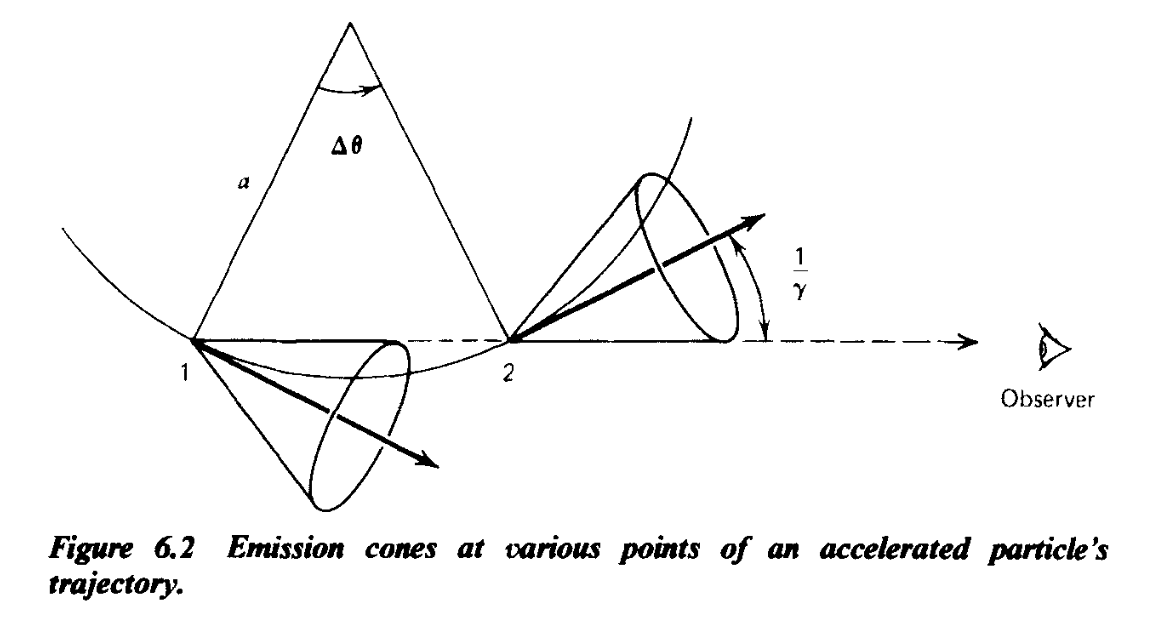
\includegraphics[width=0.75\linewidth]{Pictures/figures/rybicki_lightman_6_2.png}
    \caption{Emission cones at various points of an accelerated particle's trajectory. Taken from Rybicki \& Lightman}
    \label{fig:synchrotron_emission_cone}
\end{figure}

By looking at figure~\ref{fig:synchrotron_emission_cone}, we can see that $\Delta \theta \sim 2/\gamma \implies \Delta s = 2a/\gamma$. Likewise, the radius of the helix is given by
\[
r = \frac{v}{\omega_B \sin \varphi},
\]
where $\varphi$ is the angle between the field and the velocity (the pitch angle). Now, the beginning of the pulse occurs when the cone first passes us at $t=0$ and ends $\Delta s$ along the path later when the observer leaves the cone. This is
\[
\Delta t = \frac{2v}{\gamma \omega_B \sin \varphi}
\]
Now, the traveled distance is different by, again, $\Delta s/c$ because one edge of the beam is emitted closer and on further. Thus,
\[
\Delta t_{\rm observed} = \frac{2}{\gamma \omega_B \sin \varphi}(1-\beta).
\]
Noting that $1-\beta \approx 1/2\gamma^2$, we have
\[
\Delta t \sim \frac{1}{\gamma^3 \omega_B \sin \varphi}.
\]
This therefore defines a \textbf{critical frequency cutoff at $1/\Delta t$}. We therefore define the \textbf{synchrotron cutoff frequency} as 
\[
\omega_c = \frac{3}{2} \gamma^3 \omega_B \sin \varphi.
\]
\par
It turns out that the \textbf{electric field depends on $\theta$ only by $\gamma \theta$}, which is a manifestation of the relativistic beaming we have been talking about. \rmk{See 4.8 of Rybicki-Lightman for a detailed explaination of this assertion.} We can therefore say that
\[
E(t) \sim F(\gamma \theta(t)).
\]
It can be shown by arguments similar to those above that $\gamma \theta \propto \omega_c t$, so $E(t) \propto g(\omega_c t)$. \rmk{We're being fairly phenomenological; however, we can say at this stage that we have some constant (independent of $t$) in front of this unknown spectral function $g(\omega_c t)$. This is still enough for us to start investigating the Fourier modes.} If we expand in Fourier space,
\[
\hat{E}(\omega) \propto \int_{-\infty}^\infty g(\omega_ct) e^{i\omega t} dt = \int_{-\infty}^{\infty} g(\xi) \exp(i\omega\xi/\omega_c)\;d\xi.
\]
Now, $dW/dt d\Omega$ is proportional to the square of the fourier modes, so if we integrate over the solid angles and divide by the orbital period to get rid of any remaining time dependence, we have
\[
\frac{dW}{dt d\omega} = C_1F\left(\frac{\omega}{\omega_c}\right).
\]
By comparing this constant to the Larmour formula above, we find
\[
\boxed{
P(\omega) = \frac{\sqrt{3}}{2\pi} \frac{q^3B\sin\varphi}{mc^2} F\left(\frac{\omega}{\omega_c}\right).
}
\]
\subsection{Effective Power Laws}

Let's consider a region of frequency where $P(\omega) \propto \omega^{-k}$. It is often the case that relativistic electrons have statistical distributions which are also power-law like in the sense that
\[
N(E) dE \sim CE^{-p}\; dE
\]
over some energy band. If we therefore integrate the single particle radiation behavior over all particles at various energies, then
\[
P_{\rm tot}(\omega) \sim C\int_{\gamma_1}^{\gamma_2} P(\omega) \gamma^{-p} d\gamma \propto \int_{\gamma_1}^{\gamma_2} F\left(\frac{\omega}{\omega_c}\right) \gamma^{-p}\;d\gamma.
\]
under a change of variables $x \propto \omega/\gamma^2$, we have
\[
P_{\rm tot} \propto \omega^{-(p-1)/2} \int_{x_1}^{x_2} F(x)x^{(p-3)/2} \;dx
\]
so we conclude the very important statement that the \textbf{power law behavior of the electrons is linked to the power law of the spectrum:}
\[
k = \frac{p-1}{2}.
\]

\section{The High Energy Picture}

We have now discussed a number of highly relevant sources of emission in high energy astrophysics and we now wish to place them into perspective somewhat. we'll go through band by band and look at the relevant processes.

\subsection{Soft X-ray Emission ($E \lesssim 10\;\mathrm{keV}$)}

The soft X-ray band encompasses photon energies below about $10\;\mathrm{keV}$,
corresponding to thermal equivalents $T \lesssim 10^8\;\mathrm{K}$.
Several distinct processes can contribute in this regime:

\begin{itemize}
    \item \textbf{Blackbody emission from hot, optically thick sources.}
    For objects with surface temperatures $\gtrsim 10^6$--$10^7\;\mathrm{K}$,
    such as neutron stars or the innermost regions of accretion disks,
    thermalized radiation can extend into the soft X-ray band. The
    requirement of high temperature and optical thickness means that
    such spectra are comparatively rare.

    \item \textbf{Thermal bremsstrahlung from hot, diffuse plasmas.}
    This is the dominant emission mechanism in galaxy clusters and
    supernova remnants, where intracluster gas reaches
    $T \sim 10^7$--$10^8\;\mathrm{K}$. Because the gas is optically
    thin, photons escape directly without thermalization, producing a
    continuum spectrum characteristic of free--free emission rather than
    a blackbody.

    \item \textbf{Line emission from heavy ions.}
    Soft X-ray spectra often show rich line features from
    highly ionized elements (e.g.~Fe, O, Ne, Mg). The strength of these
    lines depends sensitively on the plasma temperature:
    \begin{itemize}
        \item At lower soft X-ray temperatures ($T \sim 10^6\;\mathrm{K}$),
              lighter elements (C, N, O) dominate.
        \item At higher temperatures ($T \gtrsim 10^7\;\mathrm{K}$),
              heavier ions (Si, S, Fe) contribute strong line complexes.
    \end{itemize}
    These lines provide powerful diagnostics of plasma temperature,
    density, and chemical composition.
\end{itemize}

\begin{remark}
    \textbf{Summary:} In the soft X-ray band, the most common emission
    mechanisms are thermal in nature: blackbody emission from very hot
    optically thick surfaces, free--free emission from hot optically
    thin plasmas, and line emission from highly ionized heavy elements.
    The relative importance of these components provides a direct probe
    of the physical state of the emitting plasma.
\end{remark}

\subsection{Hard X-ray Emission ($\sim 10$--$100\;\mathrm{keV}$)}

In the hard X-ray band, the character of emission changes
substantially compared to the soft X-ray regime. The key point is that
\textbf{thermal processes become inefficient}:

\begin{itemize}
    \item \textbf{Blackbody emission fails.}  
    To produce significant flux at $E \gtrsim 10\;\mathrm{keV}$, a
    blackbody would require temperatures $T \gtrsim 10^9\;\mathrm{K}$,
    which are rarely realized in optically thick astrophysical objects.
    As a result, blackbody radiation does not extend naturally into the
    hard band.

    \item \textbf{Thermal bremsstrahlung cutoff.}  
    The exponential factor $\exp(-h\nu/kT)$ in the free--free spectrum
    rapidly suppresses emission once $h\nu \gg kT$. Unless the plasma
    temperature exceeds $T \sim 10^8\;\mathrm{K}$, bremsstrahlung
    produces little flux in the hard band. Thus, galaxy clusters and
    supernova remnants, while bright in soft X-rays, are strongly
    suppressed here.

    \item \textbf{Emergence of non--thermal processes.}  
    In this band the dominant mechanisms are non--thermal:
    \begin{enumerate}
        \item \emph{Inverse Compton scattering (Comptonization):}
              seed photons (e.g.~UV or soft X-rays from accretion disks)
              are upscattered by hot or relativistic electrons in
              coronae, producing hard power--law tails.
        \item \emph{Non--thermal bremsstrahlung:} accelerated electrons
              colliding with ambient ions can yield a hard continuum.
    \end{enumerate}
    These processes naturally give rise to \textbf{power--law spectra}
    rather than exponential cutoffs, a hallmark of the hard X-ray band.
\end{itemize}

\begin{remark}
    \textbf{Summary:} The hard X-ray regime marks the transition from
    thermal to non--thermal astrophysics. Blackbody and thermal
    bremsstrahlung contributions are exponentially suppressed, while
    non--thermal processes such as inverse Compton scattering and
    non--thermal bremsstrahlung dominate the emission.
\end{remark}

\subsection{Low-Energy Gamma Rays ($10\;\mathrm{keV}$--$10\;\mathrm{MeV}$)}

Moving into the low-energy gamma-ray regime, additional processes
become important:

\begin{itemize}
    \item \textbf{Isomeric nuclear transitions.}  
    In addition to electron excitations, nuclei themselves can occupy
    \emph{metastable excited states}, called \emph{nuclear isomers}. Much
    like electronic fluorescence, these states may decay back to the nuclear
    ground state via the emission of a photon, but here the photon energy is
    set by nuclear rather than electronic binding energies. As a result, the
    transitions occur in the $\sim 100\;\mathrm{keV}$ to $\sim \mathrm{MeV}$
    range, producing \textbf{narrow gamma-ray lines}. These nuclear
    de-excitations are distinct from beta decay: no change in proton or
    neutron number occurs, only a rearrangement of nucleons within the same
    nucleus. 
    
    In contrast, \textbf{beta decay} involves the weak interaction and a
    transmutation of the nucleus (neutron $\to$ proton or vice versa). Many
    beta decays do leave the daughter nucleus in an excited state, which
    then de-excites by emitting gamma rays at characteristic energies. Thus
    gamma-ray lines can arise either from \emph{direct isomeric transitions}
    or from \emph{secondary de-excitations following beta decay}. In both
    cases, the resulting line features provide direct probes of
    nucleosynthesis and the isotopic composition of astrophysical sources
    (e.g.~supernova ejecta, radioactive isotopes in the interstellar medium).

    \item \textbf{Electron--positron annihilation.}  
    Pair annihilation produces the characteristic $511\;\mathrm{keV}$
    line, often accompanied by a continuum from in--flight annihilation
    or positronium formation. This process is relevant in compact object
    environments where pair plasmas can form.
\end{itemize}

\begin{remark}
    \textbf{Summary:} At low gamma-ray energies, line processes emerge
    alongside continua. Nuclear transitions yield discrete spectral
    features, while pair annihilation produces the distinct 511 keV
    line, a key diagnostic of relativistic pair plasmas.
\end{remark}

\subsection{Medium Energy Gamma Rays ($140\;\mathrm{MeV}$--$10\;\mathrm{GeV}$)}

In this band, new processes appear that are rooted in hadronic
interactions rather than atomic or nuclear transitions.

\begin{itemize}
    \item \textbf{Pion production and decay.}  
    The neutral pion has a rest mass of $m_{\pi^0} c^2 \simeq
    135\;\mathrm{MeV}$. In high--energy environments, collisions of
    relativistic protons or heavier nuclei (``cosmic rays'') with
    ambient matter can produce pions. The neutral pion rapidly decays
    via
    \[
        \pi^0 \;\to\; \gamma + \gamma,
    \]
    yielding two photons each with energies of order
    $\sim 70\;\mathrm{MeV}$ in the pion rest frame. In astrophysical
    sources, boosted pions produce broad $\gamma$--ray spectra peaking
    in the $\sim 100\;\mathrm{MeV}$--GeV range.

    \item \textbf{Charged pion channels.}  
    Charged pions ($\pi^\pm$) decay into muons and neutrinos, and the
    resulting leptons can further radiate (via synchrotron or inverse
    Compton) and contribute continuum emission in this band.

    \item \textbf{Astrophysical relevance.}  
    Medium--energy $\gamma$ rays are a \emph{smoking gun} for hadronic
    processes: detecting the characteristic ``pion bump'' around
    100--200 MeV provides direct evidence of cosmic ray protons
    colliding with ambient matter. This is a key diagnostic in supernova
    remnants, molecular clouds, and active galactic nuclei where cosmic
    ray acceleration is expected.
\end{itemize}

\begin{remark}
    \textbf{Summary:} The $140\;\mathrm{MeV}$--$10\;\mathrm{GeV}$ band
    is dominated by \emph{pion production and decay}. Neutral pions
    decay directly to gamma rays, producing a distinctive spectral
    feature, while charged pions generate leptons and neutrinos that
    feed into broader non--thermal emission channels. Observations in
    this band directly probe the hadronic component of cosmic rays.
\end{remark}


\subsection{High Energy Gamma Rays ($>10\;\mathrm{GeV}$)}

In the very high energy $\gamma$--ray regime, emission is purely
non--thermal. The dominant processes involve relativistic particle
populations interacting with background fields:

\begin{itemize}
    \item \textbf{Inverse Compton scattering.}  
    Relativistic electrons with Lorentz factor $\gamma$ can upscatter
    background photons of energy $E$ to
    \[
        E_{\rm sc} \;\sim\; \gamma^2 E,
    \]
    provided the scattering occurs in the Thomson limit
    ($E' \ll m_e c^2$ in the electron rest frame).
    For example:
    \begin{itemize}
        \item CMB photons ($E \sim 10^{-3}\,\mathrm{eV}$) scattered by
              $\gamma \sim 10^6$ electrons produce
              $E_{\rm sc} \sim 1\;\mathrm{GeV}$--TeV photons, still
              within the Thomson regime because
              $\gamma E \sim 1\;\mathrm{keV} \ll m_e c^2$.
        \item Optical/UV photons ($E \sim 1\;\mathrm{eV}$) with the same
              $\gamma \sim 10^6$ electrons would yield
              $E_{\rm sc} \sim 1\;\mathrm{TeV}$, but now
              $\gamma E \sim 1\;\mathrm{MeV} \gtrsim m_e c^2$,
              pushing the interaction into the
              \textbf{Klein--Nishina regime}, where the cross section is
              suppressed and the maximum scattered photon energy is
              limited to $\sim \gamma m_e c^2 \approx 500\;\mathrm{GeV}$.
    \end{itemize}
    Thus, inverse Compton scattering can remain efficient into the VHE
    band, but only if the seed photons are sufficiently low in energy
    (CMB, IR). For optical/UV seed fields, KN suppression becomes
    significant.

    \item \textbf{Hadronic pion decay.}  
    Relativistic protons colliding with gas produce $\pi^0$ mesons,
    which decay into $\gamma$--rays. This channel remains efficient at
    $>10\;\mathrm{GeV}$ and is often invoked to explain spectra from
    supernova remnants, AGN jets, and cosmic ray interactions in the
    interstellar medium.

    \item \textbf{Synchrotron and curvature radiation.}  
    Extremely energetic electrons in strong magnetic fields can radiate
    into the GeV--TeV range. This is important in pulsar wind nebulae,
    magnetars, and compact object magnetospheres.
\end{itemize}

\begin{remark}
    \textbf{Summary:} Above $\sim 10\;\mathrm{GeV}$, all emission is
    non--thermal. Inverse Compton scattering is efficient for low-energy
    seed photons (CMB, IR) but enters the Klein--Nishina regime for
    optical/UV/X-ray fields, reducing efficiency and altering spectral
    shapes. Hadronic pion decay and extreme synchrotron/curvature
    emission provide additional channels, making this band a key probe
    of both relativistic leptons and hadrons in astrophysical sources.
\end{remark}

